 \documentclass{article}
\usepackage[italian]{babel}
\usepackage[colorlinks=true, allcolors=blue]{hyperref}
\usepackage[a4paper,top=2cm,bottom=2cm,left=2cm,right=2cm,marginparwidth=1.75cm]{geometry}
\usepackage{adjustbox} % Pacchetto per controllare le dimensioni degli oggetti
\usepackage{graphicx} % Required for inserting images
\usepackage[inkscapeformat=png]{svg}
\usepackage{indentfirst}
\usepackage{stackengine}
\usepackage[document]{ragged2e}
\usepackage{float}
\usepackage{array}
\usepackage{tabularx}
\usepackage{subcaption}
\usepackage{hyperref} % Per rendere l'indice interagibile
\usepackage{listings}
\usepackage{xcolor}
\usepackage[export]{adjustbox}

\definecolor{codegreen}{rgb}{0,0.6,0}
\definecolor{codegray}{rgb}{0.5,0.5,0.5}
\definecolor{codepurple}{rgb}{0.58,0,0.82}
\definecolor{backcolour}{rgb}{0.95,0.95,0.92}
\definecolor{darkgreen}{rgb}{0.00,0.60,0.20}

\lstdefinestyle{SQL_CODE}{
  backgroundcolor=\color{backcolour}, commentstyle=\color{codegreen},
  keywordstyle=\color{darkgreen},
  numberstyle=\color{codegray},
  stringstyle=\color{codepurple},
  basicstyle=\ttfamily\footnotesize,
  breakatwhitespace=false,
  breaklines=true,
  captionpos=b,
  keepspaces=true,
  numbers=left,
  showspaces=false,
  showstringspaces=false,
  showtabs=false,
  tabsize=4
}

\title{Relazione progetto di laboratorio \\ Basi di dati - A.A. 2023/2024}

\author{
    Chierchia Kevin\ -
	\texttt{147798}\ -
	{chierchia.kevin@spes.uniud.it}
    \and
	Ndoye Ibrahime\ -
	\texttt{150340}\ -
	{ndoye.ibrahime@spes.uniud.it}
	\and
	Moreno Scozzi\ -
	\texttt{150356}\ -
	{scozzi.moreno@spes.uniud.it}
	}

\begin{document}
\setlength{\parindent}{25pt}
\setlength{\parskip}{5pt}
\graphicspath{{./img/}}
\maketitle
{
    \centering\href{https://github.com/kevchi9/uniud_db24}{GitHub Repository}
    \newpage
    \hypersetup{linkcolor=black}
    \tableofcontents

}

\newpage

\section{Introduzione}
Il presente elaborato espone l’attività di progettazione e implementazione di una Base di Dati relazionale, con una
successiva analisi dei dati sperimentali in essa contenuti tramite apposite interrogazioni in linguaggio SQL. \\
Di seguito elencheremo i file creati durante lo sviluppo del progetto per la creazione di database. \\

\subsection{File prodotti}
Tutto l'elaborato è stato caricato all'interno della \href{https://github.com/kevchi9/uniud_db24/}{repository github} appositamente creata per lo sviluppo di questo progetto.

\subsection{Scelte implementative}
Durante lo sviluppo sono stati usati diversi linguaggi tra cui SQL per la definizione e interrogazione delle tabelle, Python per il popolamento delle tabelle e R per la produzione di grafici.

\subsection{Scope del documento}
Lo scope principale di questo documento è quello di mostrare le fasi della progettazione di una base di dati, con un focus particolare sulla parte di analisi dei requisiti e progettazione logica. \textbf{Non} verranno trattati nel dettaglio gli argomenti del popolamento della base di dati (dunque lo sviluppo degli script Python) e dello sviluppo del codice R per la produzione dei grafici (ne verranno mostrati solo degli estratti). 
\section{Analisi dei requisiti}

\subsection{Requisiti}

Si vuole progettare una base di dati di supporto alla gestione degli interventi di assistenza clienti effettuati da un’azienda che opera nell’ambito degli impianti di riscaldamento.\\

\noindent\fbox{%
    \setlength{\fboxrule}{0.1pt}
    \parbox{\textwidth}{%
        \begin{itemize}
            \item L’azienda possiede un certo numero di \textbf{\underline{clienti}}, appartenenti a diverse categorie (\underline{aziende}, \underline{enti pubblici}, \underline{singoli cittadini}, ..). 
            Di ogni \underline{cliente}, identificato da uno specifico codice, l’azienda possiede indirizzo, recapito telefonico ed estremi della persona di riferimento.
            
            \item Ogni \underline{cliente} può formulare una \textbf{\underline{richiesta}} di assistenza attraverso appositi moduli disponibili on-line. Ogni \underline{richiesta} è identificata univocamente da un codice numerico generato automaticamente dal sistema. In ogni \underline{richiesta}, il \underline{cliente} deve specificare il sistema per il quale richiede l’intervento di assistenza e la tipologia del problema (scegliendola in un insieme predefinito di tipologie).
            
            \item Ad ogni \underline{richiesta} di assistenza da parte di un \underline{cliente}, corrispondono uno o più \textbf{\underline{interventi}} di assistenza da parte dell’azienda. Ogni \underline{intervento} relativo ad una data \underline{richiesta} è identificato da un numero progressivo (intervento 1 relativo alla richiesta 734, intervento 2 relativo alla richiesta 734, ..). Gli \underline{interventi} possono essere svolti sia \underline{in remoto} (il \underline{cliente} viene contattato telefonicamente e il problema viene risolto attraverso tale interazione) o \underline{presso la sede} del \underline{cliente}. Di ogni \underline{intervento} vengono registrati il giorno in cui ha luogo (si assume che ogni \underline{intervento} venga eseguito in giornata) e la durata.
            
            \item Ogni \underline{intervento} viene effettuato da un \textbf{\underline{tecnico}} dell’azienda. Se una \underline{richiesta} di assistenza comporta l’esecuzione di più \underline{interventi}, questi possono essere svolti da \underline{tecnici} diversi. Ogni \underline{tecnico} è identificato univocamente dal suo codice fiscale. Per ogni \underline{tecnico} vengono specificate le tipologie di problemi che è in grado di risolvere (tali tipologie appartengono ad un insieme predefinito di possibili tipologie). L’esecuzione di un \underline{intervento} relativo ad una data \underline{richiesta} deve ovviamente essere assegnata ad un \underline{tecnico} che ha le competenze necessarie (corrispondenza tra tipologia del problema specificata nella \underline{richiesta} e tipologie di problemi per i quali il \underline{tecnico} ha le competenze necessarie).

        \end{itemize}
    }%
}

Il \textbf{dominio applicativo} della base di dati è l'\textbf{azienda} di impianti di riscaldamento.

\subsection{Glossario}

La traccia assegnata contiene i seguenti termini appartenenti al dominio di interesse relativo a un'azienda di impianti di riscaldamento:

\begin{table}[h!]
    \centering
    \begin{adjustbox}{width=1\textwidth}
        \begin{tabular}{|c|c|c|c|}
            \hline &&& \\ 
            \textbf{Termine} & \textbf{Descrizione} & \textbf{Attributi} & \textbf{Collegamenti} \\ &&& \\ 
            \hline &&& \\ 
            Cliente & Persona che richiede interventi di assistenza. & \underline{\textbf{ID}}, indirizzo, telefono, persona di riferimento  & Richiesta \\ &&& \\
            \hline &&& \\ 
            Richiesta & Richiesta di intervento per la risoluzione di un problema. & \underline{\textbf{Codice}}, sistema interessato, tipo problema  & Cliente, Intervento\\ &&& \\ 
            \hline &&& \\ 
            Intervento & Azione di risoluzione del problema da parte di un tecnico. & \underline{\textbf{Richiesta, numero intervento}} & Richiesta, Tecnico\\ &&& \\ 
            \hline &&& \\ 
            Tecnico & Dipendente incaricato della risoluzione di un problema. & \underline{\textbf{CF}}, competenze & Intervento, Richiesta\\ &&& \\ 
            \hline
        \end{tabular}
    \end{adjustbox}
    \caption{Glossario dei termini}
    \label{tab:glossario}
\end{table}

\newpage

\subsection{Ristesura e strutturazione dei requisiti}

In seguito all'identificazione dei termini chiave, si raccolgono i requisiti espressi in linguaggio naturale in maniera più strutturata. Tale organizzazione può tornare utile in fase progettazione, nell'assegnamento delle responsabilità.

\begin{table}[h]
    \centering
    \begin{tabular}{|m{17cm}|}
        \hline
        \begin{center} \textbf{Cliente} \end{center} \\
        \hline
        \begin{itemize}
            \item appartenente a diverse categorie (aziende, enti pubblici, singoli cittadini, ..)
            \item identificato da uno specifico codice, indirizzo, recapito telefonico, estremi della persona di riferimento (\textbf{nel caso in cui sia un'azienda})
            \item può formulare richieste, per ognuna delle quali deve specificare il sistema per il quale richiede l'intervento e il tipo di problema
        \end{itemize} \\
        
        \hline
        \begin{center}\textbf{Richiesta}\end{center} \\
        \hline
        \begin{itemize}
            \item identificata univocamente da un codice numerico
            \item per ogni richiesta è specificato il sistema per il quale è richiesto l'intervento
            \item ad ogni richiesta corrispondono uno o più interventi
        \end{itemize} \\
        
        \hline
        \begin{center}\textbf{Intervento}\end{center} \\
        \hline
        \begin{itemize}
            \item identificato da un numero progressivo relativo alla richiesta che lo genera
            \item possono essere svolti in remoto o in loco
            \item di ogni intervento si registra il giorno e la durata
            \item ad ogni intervento corrisponde un solo tecnico
        \end{itemize} \\
        
        \hline
        \begin{center}\textbf{Tecnico}\end{center} \\
        \hline
        \begin{itemize}
            \item identificato dal suo codice fiscale
            \item più tecnici possono essere coinvolti per un'unica richiesta (in caso di interventi multipli)
            \item a un tecnico possono essere assegnati solo interventi la cui tipologia corrisponde alle sue competenze 
        \end{itemize} \\
        \hline
    \end{tabular}
    \caption{Requisiti strutturati}
    \label{tab:op_freq}
\end{table}

\newpage

\subsection{Operazioni sui dati}

Individuati i requisiti, si descrivono ora le principali operazioni sui dati, con la rispettiva frequenza.
Si ipotizza, per dare consistenza al conteggio, un'azienda con 100 clienti attivi, 5 tecnici e una stima di 20 guasti mensili con conseguenti richieste di interventi.

\begin{table}[h]
    \centering
    \begin{tabular}{|m{10cm} m{3cm}|}
        \hline 
        \textbf{Operazione} & \textbf{Frequenza} \\ 
        
        \hline & \\   
        Inserimento di un nuovo Cliente & 10/mese \\&\\

        Visualizzazione dei dettagli di un Cliente & 50/mese \\&\\
        
        Inserimento di una Richiesta & 20/mese \\&\\
        
        Visualizzazione dei dettagli di una Richiesta & 200/mese \\&\\

        Inserimento di un Intervento & 40/mese \\&\\

        Visualizzazione dei dettagli di un Intervento & 80/mese \\&\\

        Visualizzazione dei dettagli di un Tecnico & 70/mese \\&\\

        \hline
    
    \end{tabular}
    \caption{Operazioni e frequenze}
    \label{tab:my_label}
\end{table}

\subsubsection{Alcuni chiarimenti}

L'elevata frequenza delle operazioni di visualizzazione di dettagli di Richiesta, Tecnico e Intervento è giustificata dal fatto che al fine ultimo di gestire le richieste e organizzare gli interventi, gli operatori che utilizzano l'applicazione che si interfaccia alla base di dati si trovino più volte ad accedere a tali dati, così come i tecnici per visualizzare i dettagli di una richiesta.
\newpage

\section{Progettazione concettuale}

\subsection{Diagramma ER}
Segue lo schema Entità-Relazione creato sulla base dei requisiti definiti precedentemente.

\begin{figure}[h]
    \centering
    \includegraphics[scale=0.25]{img/ER_base_definitivo.png}
    \label{fig:ER_Schema1}
\end{figure}

    \subsubsection{Vincoli di integrità}
    Dalla consegna si evince un evidente vincolo di integrità \textbf{tra le entità Tecnico e Richiesta}: \\ al momento dell'inserimento di una richiesta, il cliente inserisce anche il \textbf{tipo ti problema} da risolvere. Tale campo può essere inserito con un insieme specifico di valori (ad esempio: \{elettrico, idraulico, ... \}), il quale è anche il \textbf{dominio del attributo 'campo competenze' di Tecnico}. \\ Dunque affinchè un intervento possa essere assegnato a uno specifico tecnico, \textbf{campo competenze di Tecnico e tipo problema di Richiesta devono combaciare}.
    
    \subsubsection{Regole di derivazione}
    
    Il diagramma presenta i seguenti attributi derivati:
    \begin{enumerate}
        \item \textbf{Numero di Richieste}: la somma di tutte le richieste effettuate da un cliente
        \item \textbf{Numero di Interventi}: la somma di tutti gli interventi forniti da una richiesta
        \item \textbf{disponibile} (Tecnico): un valore booleano che rappresenta la disponibilità del tecnico. È vero se il tecnico non è già impegnato in un altro intervento. Si deriva da data e durata di Intervento.
        \item \textbf{tel. cliente} (Intervento remoto): si deriva dal numero di telefono del cliente.
    \end{enumerate}

\subsection{Alcune osservazioni}
Sulla base delle specifiche dei requisiti, si evince che Intervento è identificato univocamente da un numero sequenziale e dalla richiesta che lo ha fornito, e di conseguenza è un \textbf{entità debole}. Dunque la chiave primaria di intervento sarà proprio la coppia n.intervento, Richiesta.

\section{Progettazione logica}
Lo scopo di questa sezione è di produrre uno schema relazionale, sulla base dello schema entità-relazione precedentemente definito. In primo luogo verrà effettuata un'analisi delle ridondanze, e in seguito una ristesura dello schema ER in preparazione allo schema relazione.

\subsection{Analisi delle ridondanze}
Al fine di decidere se mantenere o eliminare le ridondanze presenti nello schema Entità-Relazione proposto in precedenza, si definisce la tavola dei volumi di entità e relazioni.
Consideriamo il caso della base di dati \underline{\textbf{dopo 3 anni di attività}}, ipotizzando uno stato iniziale, come detto al punto 2.4, di 100 clienti attivi, 5 tecnici e 20 guasti mensili. Si ipotizza inoltre che nell'arco dei 3 anni siano aumentati anche i tecnici (uno all'anno). 

\begin{table}[h]
    \centering
    \begin{adjustbox}{width=1\textwidth}
        \begin{tabular}{|m{5cm}|m{5cm}|m{3cm}|}
            \hline  
            \textbf{Concetto} & \textbf{Tipo} & \textbf{Volume} \\ 
            \hline
            Cliente & Entità & 460 \\ 
            \hline
            Richiesta & Entità & 720 \\
            \hline
            Intervento & Entità & 1440 \\
            \hline
            Tecnico & Entità & 8 \\
            \hline
            Effettua & Relazione & 720 \\
            \hline
            Fornisce & Relazione & 1440\\
            \hline
            è assegnato a & Relazione & 1440 \\
            \hline
        \end{tabular}
    \end{adjustbox}
    \caption{Volume dei dati}
    \label{tab:volumetable}
\end{table}

\subsubsection{Attributi derivabili}

Per come è stato definito il diagramma ER, sappiamo che sono presenti quattro attributi derivati: \\ \textbf{Numero di Richieste}, \textbf{Numero di Interventi}, \textbf{tel. cliente} e \textbf{disponibile}.\\
Nei punti successivi verranno analizzati uno ad uno.

\newpage

\subsection{Attributo Numero di Richieste}

La ridondanza introdotta dall'attributo Numero di Richiesta coinvolge principalmente due operazioni:
\begin{enumerate}
    \item \underline{Inserimento di una Richiesta}
    \item \underline{Visualizzazione dei dettagli di un Cliente}
\end{enumerate}

\subsubsection{Tabelle degli accessi}

Si producono le tabelle degli accessi delle operazioni sopracitate con e senza ridondanza.

\textbf{Con ridondanza}

\begin{table}[h]
    \centering
    \begin{adjustbox}{width=0.6\textwidth}
        \begin{tabular}{|m{2cm}|m{2cm}|m{2cm}|m{2cm}|}
            \hline  
            \textbf{Concetto} & \textbf{Tipo} & \textbf{Accessi} & \textbf{Tipo}\\ 
            \hline
            Richiesta & E & 1 & W\\
            \hline
            Effettua & R & 1 & W\\
            \hline
            Cliente & E & 1 & R\\
            \hline
            Cliente & E & 1 & W\\
            \hline
        \end{tabular}
    \end{adjustbox}
    \caption{Tabella degli accessi per "Inserimento di una Richiesta" }
    \label{tab:accesstable1}
\end{table}

\begin{table}[h]
    \centering
    \begin{adjustbox}{width=0.6\textwidth}
        \begin{tabular}{|m{2cm}|m{2cm}|m{2cm}|m{2cm}|}
            \hline  
            \textbf{Concetto} & \textbf{Tipo} & \textbf{Accessi} & \textbf{Tipo}\\ 
            \hline
            Cliente & E & 1 & R\\
            \hline
        \end{tabular}
    \end{adjustbox}
    \caption{Tabella degli accessi per "Visualizzazione dei dettagli di un Cliente"}
    \label{tab:accesstable2}
\end{table}

\textbf{Senza ridondanza}

\begin{table}[h]
    \centering
    \begin{adjustbox}{width=0.6\textwidth}
        \begin{tabular}{|m{2cm}|m{2cm}|m{2cm}|m{2cm}|}
            \hline  
            \textbf{Concetto} & \textbf{Tipo} & \textbf{Accessi} & \textbf{Tipo}\\ 
            \hline
            Richiesta & E & 1 & W\\
            \hline
            Effettua & R & 1 & W\\
            \hline
        \end{tabular}
    \end{adjustbox}
    \caption{Tabella degli accessi per "Inserimento di una Richiesta" }
    \label{tab:accesstable3}
\end{table}

\begin{table}[h!]
    \centering
    \begin{adjustbox}{width=0.6\textwidth}
        \begin{tabular}{|m{2cm}|m{2cm}|m{2cm}|m{2cm}|}
            \hline  
            \textbf{Concetto} & \textbf{Tipo} & \textbf{Accessi} & \textbf{Tipo}\\ 
            \hline
            Cliente & E & 1 & R\\
            \hline
            Effettua & R & 1,5 & R\\
            \hline
        \end{tabular}
    \end{adjustbox}
    \caption{Tabella degli accessi per "Visualizzazione dei dettagli di un Cliente"}
    \label{tab:accesstable4}
\end{table}

\subsubsection{Analisi dei costi mensili}

\begin{itemize}
    \item \textbf{Con ridondanza}:
    \begin{enumerate}
        \item Inserimento di una Richiesta(20/mese): si hanno 60 accessi in scrittura e 20 in lettura, per un totale di \textbf{140} accessi.
        \item Visualizzazione dei dettagli di un Cliente(50/mese): si hanno solo \textbf{50} accessi in lettura.
    \end{enumerate}
    \item \textbf{Senza ridondanza}:
    \begin{enumerate}
        \item Inserimento di una Richiesta(20/mese): si hanno 40 accessi in scrittura, per un totale di \textbf{80} accessi.
        \item Visualizzazione dei dettagli di un Cliente(50/mese): si hanno solo \textbf{125} accessi in lettura.
    \end{enumerate}
\end{itemize}

\subsubsection{Conclusioni}

Nel caso con ridondanza si hanno 190 accessi contro 205 del caso senza ridondanza, risulta dunque conveniente mantenere l'attributo Numero di Richieste in Cliente.

\newpage

\subsection{Attributo Numero di Interventi}

La ridondanza introdotta dall'attributo Numero di Interventi coinvolge invece due operazioni:
\begin{enumerate}
    \item \underline{Inserimento di un Intervento}
    \item \underline{Visualizzazione dei dettagli di una Richiesta}
\end{enumerate}

\subsubsection{Tabelle degli accessi }
In seguito le tabelle degli accessi per le operazioni sopracitate con e senza ridondanza.

\textbf{Con ridondanza}

\begin{table}[h]
    \centering
    \begin{adjustbox}{width=0.6\textwidth}
        \begin{tabular}{|m{2cm}|m{2cm}|m{2cm}|m{2cm}|}
            \hline  
            \textbf{Concetto} & \textbf{Tipo} & \textbf{Accessi} & \textbf{Tipo}\\ 
            \hline
            Intervento & E & 1 & W\\
            \hline
            Fornisce & R & 1 & W\\
            \hline
            Richiesta & E & 1 & R\\
            \hline
            Richiesta & E & 1 & W\\
            \hline            
        \end{tabular}
    \end{adjustbox}
    \caption{Tabella degli accessi per Inserimento di un Intervento}
    \label{tab:accesstable5}
\end{table}

\begin{table}[h]
    \centering
    \begin{adjustbox}{width=0.6\textwidth}
        \begin{tabular}{|m{2cm}|m{2cm}|m{2cm}|m{2cm}|}
            \hline  
            \textbf{Concetto} & \textbf{Tipo} & \textbf{Accessi} & \textbf{Tipo}\\ 
            \hline
            Richiesta & E & 1 & R\\
            \hline            
        \end{tabular}
    \end{adjustbox}
    \caption{Tabella degli accessi per Visualizzazione dei dettagli di una Richiesta}
    \label{tab:accesstable6}
\end{table}

\textbf{Senza ridondanza}

\begin{table}[h]
    \centering
    \begin{adjustbox}{width=0.6\textwidth}
        \begin{tabular}{|m{2cm}|m{2cm}|m{2cm}|m{2cm}|}
            \hline  
            \textbf{Concetto} & \textbf{Tipo} & \textbf{Accessi} & \textbf{Tipo}\\ 
            \hline
            Intervento & E & 1 & W\\
            \hline
            Fornisce & R & 1 & W\\
            \hline
        \end{tabular}
    \end{adjustbox}
    \caption{Tabella degli accessi per Inserimento di un Intervento}
    \label{tab:accesstable7}
\end{table}

\begin{table}[h!]
    \centering
    \begin{adjustbox}{width=0.6\textwidth}
        \begin{tabular}{|m{2cm}|m{2cm}|m{2cm}|m{2cm}|}
            \hline  
            \textbf{Concetto} & \textbf{Tipo} & \textbf{Accessi} & \textbf{Tipo}\\ 
            \hline
            Richiesta & E & 1 & R\\
            \hline
            Fornisce & R & 2 & R\\
            \hline
        \end{tabular}
    \end{adjustbox}
    \caption{Tabella degli accessi per Visualizzazione dei dettagli di una Richiesta}
    \label{tab:accesstable8}
\end{table}

\subsubsection{Analisi dei costi mensili}

\begin{itemize}
    \item \textbf{Con ridondanza}:
    \begin{enumerate}
        \item \textbf{Inserimento di un Intervento}(40/mese): si hanno 120 accessi in scrittura e 40 accessi in lettura, per un totale di \textbf{280} accessi.
        \item \textbf{Visualizzazione dei dettagli di una Richiesta}(200/mese): si hanno solo \textbf{200} accessi in lettura.
    \end{enumerate}
    \item \textbf{Senza ridondanza}:
    \begin{enumerate}
        \item \textbf{Inserimento di un Intervento}(40/mese): si hanno 80 accessi in scrittura per un totale di \textbf{160} accessi.
        \item \textbf{Visualizzazione dei dettagli di una Richiesta}(200/mese): si hanno solo \textbf{600} accessi in lettura.
    \end{enumerate}
\end{itemize}

\subsubsection{Conclusioni}

Nel caso con ridondanza si hanno 480 accessi contro 760 del caso senza ridondanza, risulta dunque conveniente mantenere l'attributo Numero di Interventi in Richiesta.

\subsection{Attributo tel. cliente}

La ridondanza introdotta dall'attributo "tel. cliente" coinvolge principalmente 2 operazioni: 

\begin{enumerate}
    \item \underline{Inserimento di Intervento}
    \item \underline{Visualizzazione dei dettagli di un Intervento} 
\end{enumerate}

\subsubsection{Tabelle degli accessi}

In seguito le tabelle degli accessi per le operazioni sopracitate con e senza ridondanza.

\textbf{Con ridondanza}\\
Per chiarezza si aggiunge alla tabella degli accessi una colonna per discriminare gli accessi che sono inclusi nel normale inserimento senza l'attributo da quelli che servono solo al popolamento dell'attributo:
    
\begin{table}[h]
    \centering
        \begin{adjustbox}{width=0.8\textwidth}
            \begin{tabular}{|m{2cm}|m{2cm}|m{2cm}|m{2cm}|m{3cm}|}
                \hline  
                \textbf{Concetto} & \textbf{Tipo} & \textbf{Accessi} & \textbf{Tipo} & \textbf{Note}\\ 
                \hline
                Intervento & E & 1 & W & Inserimento \\
                \hline
                Fornisce & R & 1 & W & Inserimento \\
                \hline
                Fornisce & R & 1 & R & Modifica attributo \\
                \hline
                Richiesta & E & 1 & R & Modifica attributo \\
                \hline
                Effettua & R & 1 & R & Modifica attributo \\
                \hline
                Cliente & E & 1 & R & Modifica attributo \\
                \hline            
                Intervento & E & 1 & W & Modifica attributo \\
                \hline
            \end{tabular}
        \end{adjustbox}
    \caption{Tabella degli accessi per Inserimento di un Intervento}
    \label{tab:accesstable9}
\end{table}

\begin{table}[h]
    \centering
        \begin{adjustbox}{width=0.6\textwidth}
            \begin{tabular}{|m{2cm}|m{2cm}|m{2cm}|m{2cm}|}
                \hline  
                \textbf{Concetto} & \textbf{Tipo} & \textbf{Accessi} & \textbf{Tipo}\\ 
                \hline
                Intervento & E & 1 & R\\
                \hline
            \end{tabular}
        \end{adjustbox}
    \caption{Tabella degli accessi per Visualizzazione dei dettagli di un Intervento}
    \label{tab:accesstable10}
\end{table}

\textbf{Senza ridondanza}

\begin{table}[h]
    \centering
        \begin{adjustbox}{width=0.6\textwidth}
            \begin{tabular}{|m{2cm}|m{2cm}|m{2cm}|m{2cm}|}
                \hline  
                \textbf{Concetto} & \textbf{Tipo} & \textbf{Accessi} & \textbf{Tipo} \\ 
                \hline
                Intervento & E & 1 & W \\
                \hline
                Fornisce & R & 1 & W \\
                \hline
            \end{tabular}
        \end{adjustbox}
    \caption{Tabella degli accessi per Inserimento di un Intervento}
    \label{tab:accesstable11}
\end{table}

\begin{table}[h!]
    \centering
        \begin{adjustbox}{width=0.6\textwidth}
            \begin{tabular}{|m{2cm}|m{2cm}|m{2cm}|m{2cm}|}
                \hline  
                \textbf{Concetto} & \textbf{Tipo} & \textbf{Accessi} & \textbf{Tipo} \\ 
                \hline
                Intervento & E & 1 & R \\
                \hline
                Fornisce & R & 1 & R \\
                \hline
                Richiesta & E & 1 & R \\
                \hline
                Effettua & R & 1 & R \\
                \hline
                Cliente & E & 1 & R \\
                \hline
            \end{tabular}
        \end{adjustbox}
    \caption{Tabella degli accessi per Visualizzazione dei dettagli di un Intervento}
    \label{tab:accesstable12}
\end{table}

\subsubsection{Analisi dei costi mensili}

\begin{itemize}
    \item \textbf{Con ridondanza}:
    \begin{enumerate}
        \item \textbf{Inserimento di un Intervento}(40/mese): si hanno 120 accessi in scrittura e 160 accessi in lettura, per un totale di \textbf{400} accessi.
        \item \textbf{Visualizzazione dei dettagli di un Intervento}(80/mese): si hanno solo \textbf{80} accessi in lettura.
    \end{enumerate}
    \newpage
    \item \textbf{Senza ridondanza}:
    \begin{enumerate}
        \item \textbf{Inserimento di un Intervento}(40/mese): si hanno 80 accessi in scrittura per un totale di \textbf{160} accessi.
        \item \textbf{Visualizzazione dei dettagli di un Intervento}(80/mese): si hanno solo \textbf{400} accessi in lettura.
    \end{enumerate}
\end{itemize}

\subsubsection{Conclusioni}

Nel caso con ridondanza si hanno 480 accessi contro 560 del caso senza ridondanza, risulta dunque conveniente mantenere l'attributo tel. cliente in Intervento.

\subsection{Attributo disponibile}

L'attributo disponibile serve a riconoscere direttamente dalla tabella Tecnico quale tecnico è disponibile. In alternativa, senza tale ridondanza vi è la necessità di cercare in "è assegnato a" una tupla contenente il tecnico da controllare e un intervento con i valori di data e durata che si sovrappongano a quelli del nuovo intervento. La presenza di tale tupla si traduce nella non disponibilità del tecnico. L'attributo coinvolge l'operazione \underline{Inserimento di un Intervento}.

\subsubsection{Tabelle degli accessi}
Poichè il controllo del campo competenze viene effettuato sia con presenza di ridondanza che non, viene omesso dal conteggio degli accessi. 

\textbf{Con ridondanza}

\begin{table}[h!]
    \centering
        \begin{adjustbox}{width=1\textwidth}
            \begin{tabular}{|m{2,2cm}|m{2cm}|m{2cm}|m{2cm}|m{6cm}|}
                \hline  
                \textbf{Concetto} & \textbf{Tipo} & \textbf{Accessi} & \textbf{Tipo} & \textbf{Note}\\ 
                \hline
                Tecnico & E & 1 & R & Ricerca candidato \\
                \hline
                Tecnico & E & 1 & W & Modifica attributo (disponibile=False)\\
                \hline
                Intervento & E & 1 & W & Inserimento \\
                \hline
                è assegnato a & R & 1 & W & Inserimento \\
                \hline
                Tecnico & E & 1 & W & Modifica attributo (disponibile=True)\\
                \hline
            \end{tabular}
        \end{adjustbox}
    \caption{Tabella degli accessi per Inserimento di un Intervento}
    \label{tab:accesstable13}
\end{table}

La seconda modifica dell'attributo (disponibile=True) avviene quando l'Intervento è terminato.

\textbf{Senza ridondanza}

\begin{table}[h]
    \centering
        \begin{adjustbox}{width=0.6\textwidth}
            \begin{tabular}{|m{2,2cm}|m{2cm}|m{2cm}|m{2cm}|}
                \hline  
                \textbf{Concetto} & \textbf{Tipo} & \textbf{Accessi} & \textbf{Tipo} \\ 
                \hline
                è assegnato a & R & 1 & R \\
                \hline
                Intervento & E & 1 & W \\
                \hline
                è assegnato a & R & 1 & W \\
                \hline
            \end{tabular}
        \end{adjustbox}
    \caption{Tabella degli accessi per Inserimento di un Intervento}
    \label{tab:accesstable14}
\end{table}

\subsubsection{Analisi dei costi mensili}

\begin{itemize}
    \item \textbf{Con ridondanza}:
    \begin{enumerate}
        \item \textbf{Inserimento di un Intervento}(40/mese): si hanno 160 accessi in scrittura e 40 in lettura, per un totale di 360 accessi 
    \end{enumerate}
    \item \textbf{Senza ridondanza}:
    \begin{enumerate}
        \item \textbf{Inserimento di un Intervento}(40/mese): si hanno 80 accessi in scrittura e 40 in lettura, per un totale di 200 accessi 
    \end{enumerate}
\end{itemize}

\subsubsection{Conclusioni}

Risulta dunque molto conveniente rimuovere l'attributo.

\subsection{Gestione delle generalizzazioni}

Nel diagramma ER, data la consegna del problema, sono state inserite \textbf{due generalizzazioni}: quella relativa a \textbf{Cliente}, che si specializza in Organizzazione e Persona, e quella di \textbf{Intervento} che si specializza in Intervento remoto e Intervento in loco.

Data la semplicità delle specializzazioni, una possibile soluzione alla codifica delle generalizzazioni nel modello relazionale è l'\textbf{eliminazione dei nodi figlio}, con il nodo genitore che ne assorbe gli attributi. In breve, eliminiamo Organizzazione e Persona nel caso di Cliente, aggiungendo a Cliente l'attributo "persona di riferimento" come \textbf{attributo opzionale} (può avere valore null).
La stessa logica viene applicata anche alla generalizzazione su Intervento: rimuoviamo le due specializzazioni e aggiungiamo l'attributo "tel. cliente" a Intervento, anche in questo caso, \textbf{senza} la clausola \textbf{not null}.

Entrambi questi attributi potranno essere popolati nel caso in cui tali entità dovessero essere un Organizzazione o un Intervento remoto.



\subsection{Revisione di Entità e Relazioni}

\subsubsection{Reifica delle relazioni}

Nel diagramma sono presenti 3 relazioni binarie:

\begin{enumerate}
    \item \textbf{Effettua} - relazione \underline{uno a molti} tra Cliente (0,N) e Richiesta (1,1) con partecipazione \underline{opzionale}
    \item \textbf{Fornisce} - relazione \underline{uno a molti} tra Intervento (1,1) e Richiesta (1,N)
    \item \textbf{è assegnato a} - relazione \underline{uno a molti} tra Tecnico (0,N) e Intervento (1,1) con partecipazione \underline{opzionale}
\end{enumerate}

Data l'assenza di relazioni molti a molti non è necessaria nessuna reifica. Tuttavia, l'entità Intervento (entità debole), avrebbe in totale 6 attributi senza creare nuove tabelle, dunque per una migliore leggibilità dei dati, è stato deciso di reificare la relazione "è assegnato a". L'entità ottenuta dalla reificazione viene rinominata in "\textbf{Registro\_interventi}" i cui record saranno identificati dalla chiave Tecnico e Intervento con i quali sarà in relazione attraverso le 2 nuove relazioni T-R e R-I.

Non sono invece presenti relazioni ternarie.

\subsubsection{Reifica degli attributi multivalore}
Nel diagramma è presente un attributo multivalore: Campo competenze di Tecnico. Questo viene dunque reificato nell'entità Competenza e unito all'entità Tecnico con la relazione Possiede.

\newpage

\subsection{Diagramma ER ristrutturato}

\begin{figure}[h]
    \centering
    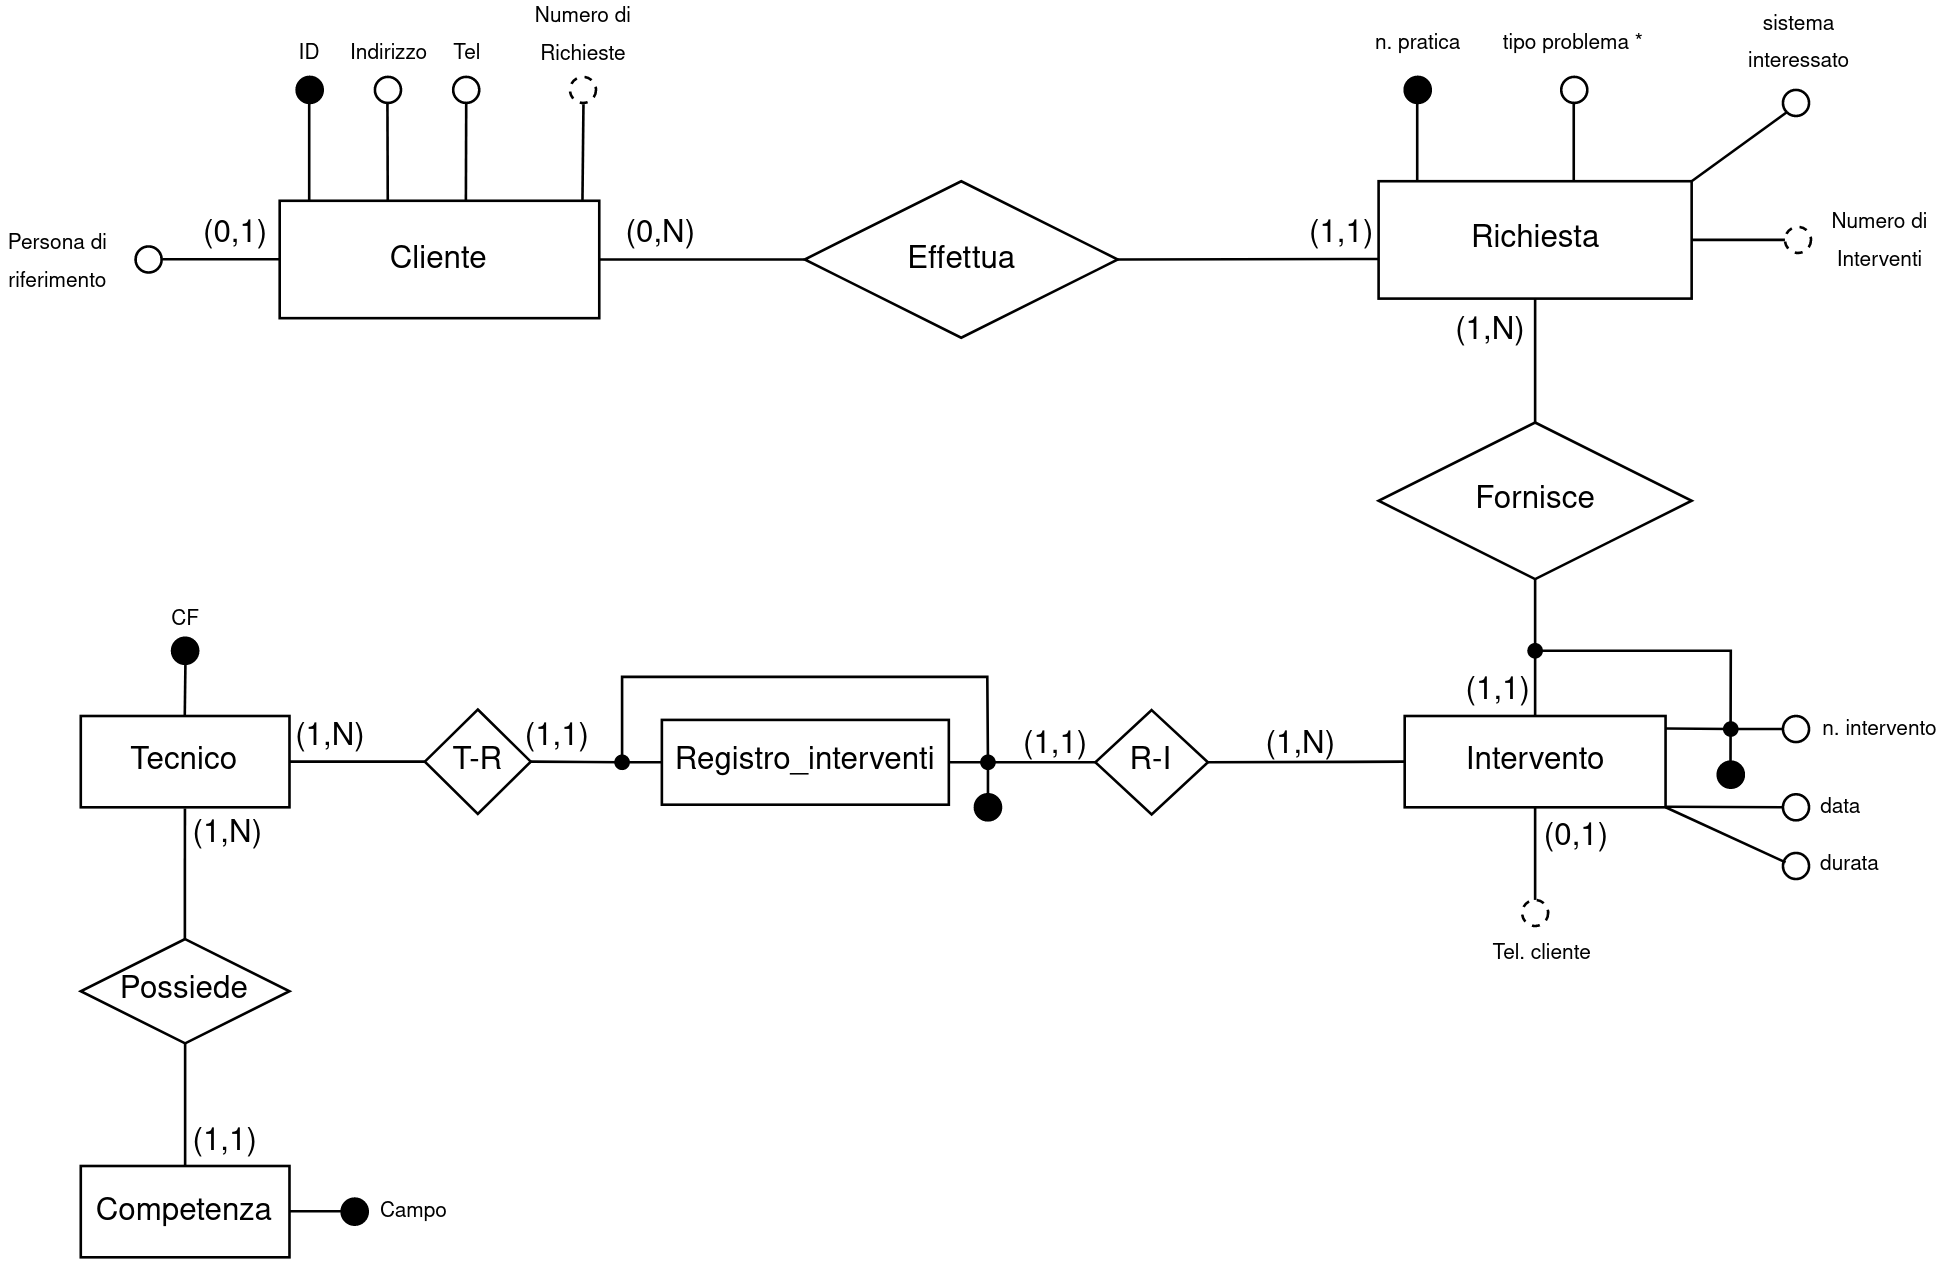
\includegraphics[scale=0.22]{img/ER_FINALE.png}
    \label{fig:ER_Schema2}
\end{figure}

\subsection{Traduzione dello schema ER in schema relazionale}

In seguito a tutte le scelte progettuali fatte nei punti precedenti, e utilizzando il diagramma ER ristrutturato, si procede alla traduzione nello schema relazionale.
Nello specifico segue la traduzione delle entità e delle sole relazioni uno a molti, in quanto non ve ne sono di altri tipi.

\subsubsection{Traduzione delle entità}
Di seguito sono riportate le entità con i rispettivi vincoli applicati sugli attributi. 
Saranno introdotte delle modifiche per codificare le relazioni non reificate, utilizzando la keyword "Modifica". 
\\Si danno per scontato i vincoli Unique e NotNull sulle \underline{chiavi} (gli attributi sottolineati).

\begin{itemize}
    \item \textbf{Cliente}(\underline{ID}, Indirizzo, Tel, PersonaDiRiferimento, NumeroDiRichieste) 
        \begin{itemize}
            \item NotNull: Indirizzo, Tel, NumeroDiRichieste
        \end{itemize}
    \item \textbf{Richiesta}(\underline{nPratica}, \textit{TipoProblema}, SistemaInteressato, \textit{Cliente}, NumeroDiInterventi
        \begin{itemize}
            \item NotNull: TipoProblema, SistemaInteressato, Cliente
            \item Chiave Esterna: Cliente si riferisce alla chiave primaria dell'entità Cliente, TipoProblema si riferisce alla chiave primaria dell'entità Competenza
            \item Modifica: Cliente è utilizzato per codificare la partecipazione alla relazione Effettua
        \end{itemize}
    \item \textbf{Intervento}(\underline{nIntervento, \textit{Richiesta}}, Data, Durata, TelCliente)
        \begin{itemize}
            \item NotNull: Richiesta, Data, Durata
            \item Chiave Esterna: Richiesta si riferisce alla chiave primaria dell'entità Richiesta
        \end{itemize}
    \item \textbf{Registro\_interventi}(\underline{\textit{Tecnico}, \textit{Richiesta}, \textit{Intervento}})
        \begin{itemize}
        \item Chiave Esterna: Tecnico si riferisce alla chiave primaria dell'entità Tecnico, Richiesta si riferisce alla chiave primaria (Richiesta) dell'entità Intervento, Intervento si riferisce alla chiave primaria (nIntervento) dell'entità Intervento
        \item Modifica: Tecnico è utilizzato per codificare la partecipazione alla relazione T-R, Intervento per codificare la partecipazione alla relazione R-I
        \end{itemize}
    \item \textbf{Tecnico}(\underline{CF})
    \item \textbf{Competenza}(\underline{Campo})
\end{itemize}
\subsubsection{Traduzioni di relazioni}
Di seguito sono riportate le relazioni con i rispettivi vincoli applicati sugli attributi.
Anche in questo caso si danno per scontati i vincoli Unique e NotNull sulle \underline{chiavi}.

\begin{itemize}
    \item \textbf{Effettua}: non reificata, viene codificata attraverso l'attributo Cliente in Richiesta.
    \item \textbf{Fornisce}: non reificata, viene codificata attraverso l'attributo Richiesta in Intervento (entità debole).
    \item \textbf{R-I}: già codificata nella reificazione di RegistroInterventi (attributo Intervento dell'entità RegistroInterventi)
    \item \textbf{T-R}: già codificata nella reificazione di RegistroInterventi (attributo Tecnico dell'entità RegistroInterventi)
    \item \textbf{Possiede}(\underline{\textit{Tecnico}, \textit{Competenza}})
    \begin{itemize}
        \item Chiave Esterna: Tecnico si riferisce alla chiave primaria dell'entità Tecnico, Competenza si riferisce alla chiave primaria dell'entità Competenza
    \end{itemize}
\end{itemize}

\subsubsection{Osservazioni}
Il vincolo di integrità indicato al punto 3.1.1, è codificato attraverso il vincolo di chiave esterna di TipoProblema in Richiesta (TipoProblema sarà dunque nello stesso dominio di Competenza).

\subsection{Schema Relazionale}

\begin{figure}[h!]
    \centering
    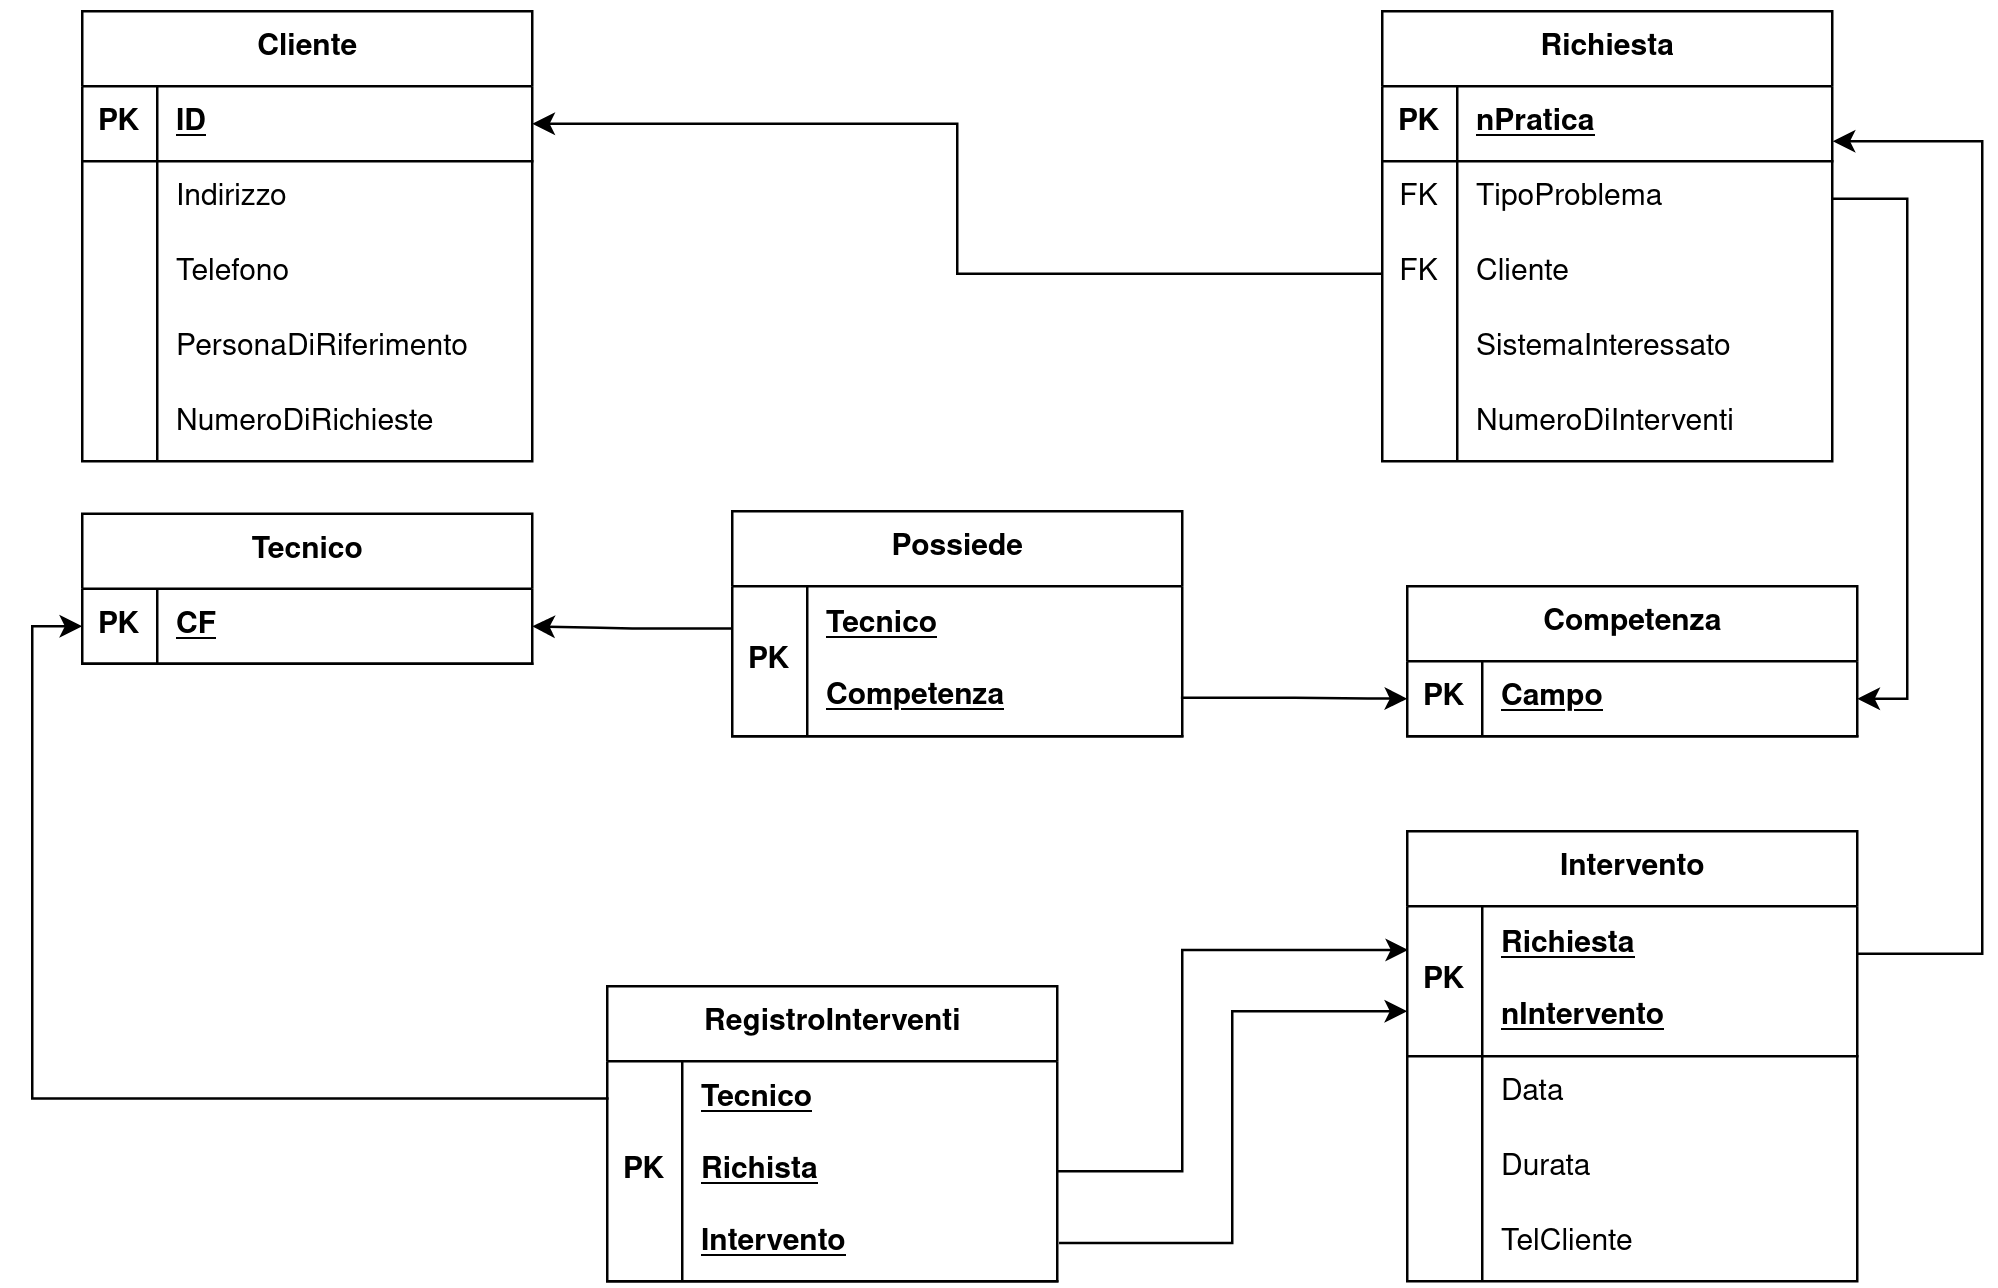
\includegraphics[scale=0.2]{img/schema_relazionale.png}
    \label{fig:ER_Schema3}
\end{figure}

\newpage
\section{Progettazione fisica}

In questa sezione verrà discussa l'implementazione in Postgres SQL del sistema progettato nei punti precedenti.
Sulla base di quanto prodotto in fase di progettazione logica 

\subsubsection{Definizione delle tabelle}

Le prime tabelle definite sono quelle prive di chiavi esterne, dunque Cliente, Tecnico e Competenza.

\lstset{style=SQL_CODE}

\begin{lstlisting}[language=SQL]
CREATE TABLE Cliente(
ID int NOT NULL PRIMARY KEY,
Indirizzo varchar(20) NOT NULL,
Tel bigint NOT NULL,
PersonaDiRiferimento varchar(20),
NumeroDiRichieste int NOT NULL);

CREATE TABLE Tecnico(
CF varchar(16) PRIMARY KEY);

CREATE TABLE Competenza(
Campo varchar(20) PRIMARY KEY);
\end{lstlisting}

Seguono ora le tabelle contenenti chiavi esterne. Per garantire l'integrità dei dati, si usa l'opzione cascade sia sugli aggiornamenti che sulle cancellazioni. Per questo motivo, sono stati anche implementati dei trigger per l'aggiornamento in caso di cancellazione degli attributi derivati definiti in precedenza.\\
Tabella Richiesta:
\begin{lstlisting}[language=SQL]
CREATE TABLE Richiesta(
nPratica int PRIMARY KEY,
TipoProblema varchar(20) NOT NULL,
Cliente int NOT NULL,
SistemaInteressato varchar(20) NOT NULL,
NumeroDiInterventi int NOT NULL,
CONSTRAINT fk_tipoProblema FOREIGN KEY (TipoProblema) 
	REFERENCES Competenza(Campo) 
	ON UPDATE CASCADE ON DELETE CASCADE,
CONSTRAINT fk_cliente FOREIGN KEY (Cliente) 
	REFERENCES Cliente(ID)
	ON UPDATE CASCADE ON DELETE CASCADE
);
\end{lstlisting}
Tabella Intervento:
\begin{lstlisting}[language=SQL]
CREATE TABLE Intervento(
Richiesta int NOT NULL,
nIntervento int NOT NULL,
Data DATE NOT NULL,
Durata interval NOT NULL,
TelCliente bigint,
PRIMARY KEY(Richiesta, nIntervento),
CONSTRAINT fk_richiesta FOREIGN KEY (Richiesta) 
	REFERENCES Richiesta(nPratica)
	ON UPDATE CASCADE
	ON DELETE CASCADE
);
\end{lstlisting}
Tabella RegistroInterventi:
\begin{lstlisting}[language=SQL]
CREATE TABLE RegistroInterventi(
Tecnico varchar(16) NOT NULL,
Richiesta int NOT NULL,
Intervento int NOT NULL,
PRIMARY KEY (Tecnico, Richiesta, Intervento),
CONSTRAINT fk_tecnico FOREIGN KEY (Tecnico) 
	REFERENCES Tecnico(CF)
	ON UPDATE CASCADE
	ON DELETE CASCADE,
CONSTRAINT fk_richiesta_intervento FOREIGN KEY (Richiesta, Intervento) 
	REFERENCES Intervento(Richiesta, nIntervento)
	ON UPDATE CASCADE
	ON DELETE CASCADE
);
\end{lstlisting}

\newpage
Tabella Possiede:
\begin{lstlisting}[language=SQL]
CREATE TABLE Possiede(
Tecnico varchar(16) NOT NULL,
Competenza varchar(20) NOT NULL,
PRIMARY KEY (Tecnico, Competenza),
CONSTRAINT fk_tecnico FOREIGN KEY (Tecnico)
	REFERENCES Tecnico(CF)
	ON UPDATE CASCADE
	ON DELETE CASCADE,
CONSTRAINT fk_competenza FOREIGN KEY (Competenza)
	REFERENCES Competenza(Campo)
	ON UPDATE CASCADE
	ON DELETE CASCADE
);
\end{lstlisting}

\subsubsection{Definizione dei trigger}

Per l'implementazione degli attributi derivati sono stati creati 4 trigger e 4 funzioni: \newline 
2 per incrementare gli attributi NumeroDiRichieste e NumeroDiInterventi in seguito a un inserimento e 
2 per decrementarli in caso di cancellazione.



\begin{lstlisting}[language=SQL]
##############################################################################
###                                                                        ###
### FUNCTION AND TRIGGER 1: UPDATE(+) nInterventi AFTER INSERT Intervento  ###
###                                                                        ###
##############################################################################

CREATE or REPLACE FUNCTION increase_numeroDiInterventi()
RETURNS TRIGGER
language plpgsql
as $$

	declare
	newValue integer;

	begin
	newValue := (SELECT (NumeroDiInterventi + 1) FROM Richiesta WHERE nPratica = new.Richiesta);
	UPDATE Richiesta SET NumeroDiInterventi = newValue WHERE nPratica = new.Richiesta;
	return new;
	end;
$$;

CREATE TRIGGER increase_counter
AFTER INSERT ON Intervento
for each row
execute procedure increase_numeroDiInterventi();

##############################################################################
###                                                                        ###
### FUNCTION AND TRIGGER 2: UPDATE(-) nInterventi BEFORE DELETE Intervento ###
###                                                                        ###
##############################################################################

CREATE or REPLACE FUNCTION decrease_numeroDiInterventi()
RETURNS TRIGGER
language plpgsql
as $$

	declare
	newValue integer;

	begin
	newValue := (SELECT (NumeroDiInterventi - 1) FROM Richiesta WHERE nPratica = old.Richiesta);
	UPDATE Richiesta SET NumeroDiInterventi = newValue WHERE nPratica = old.Richiesta;
	return old;
	end;
$$;

CREATE TRIGGER decrease_counter
AFTER DELETE ON Intervento
for each row
execute procedure decrease_numeroDiInterventi();
\end{lstlisting}

\begin{lstlisting}[language=SQL]
#############################################################################
###                                                                       ###
###  FUNCTION AND TRIGGER 3: UPDATE(+) nRichieste AFTER INSERT Richiesta  ###
###                                                                       ###
#############################################################################

CREATE OR REPLACE FUNCTION increase_numeroDiRichieste()
RETURNS TRIGGER
language plpgsql
as $$

	declare 
	newValue integer;

	begin
	newValue := (SELECT (NumeroDiRichieste + 1) FROM Cliente WHERE ID = new.Cliente);
	UPDATE Cliente SET NumeroDiRichieste = newValue WHERE ID = new.Cliente;
	return new;
	end;
$$;

CREATE TRIGGER increase_counter
AFTER INSERT ON Richiesta
for each row
execute procedure increase_numeroDiRichieste();

#############################################################################
###                                                                       ###
### FUNCTION AND TRIGGER 4: UPDATE(-) nRichieste BEFORE DELETE Richiesta  ###
###                                                                       ###
#############################################################################

CREATE OR REPLACE FUNCTION decrease_numeroDiRichieste()
RETURNS TRIGGER
language plpgsql
as $$

	declare 
	newValue integer;

	begin
	newValue := (SELECT (NumeroDiRichieste - 1) FROM Cliente WHERE ID = old.Cliente);
	UPDATE Cliente SET NumeroDiRichieste = newValue WHERE ID = old.Cliente;
	return old;
	end;
$$;

CREATE TRIGGER decrease_counter
BEFORE DELETE ON Richiesta
for each row
execute procedure decrease_numeroDiRichieste();
\end{lstlisting}

\subsection{Popolamento delle tabelle tramite script Python}

Al fine di poter manipolare e controllare al meglio i campioni da inserire nelle tabelle, sono stati implementati degli script Python. L'output ottenuto da tali script consiste in alcuni file di testo, convertibili in file .sql, contenenti comandi SQL per il popolamento della base di dati.\\ Gli script non vengono inseriti in questo documento poichè out-of-scope ma sono disponibili sulla\\ \href{https://github.com/kevchi9/uniud\_db24}{repository github}, all'interno della cartella data. \\Nella cartella SQL si trovano invece i comandi SQL illustrati nel punto precedente, e delle query usate come spunto per l'analisi dei dati.

\newpage

\section{Analisi dei dati}

L'analisi dei dati illustrata in questo capitolo è stata effettuata su una base di dati avente \textbf{1000 clienti}, \textbf{2000 richieste} con \textbf{massimo 3 interventi l'una} e \textbf{15 tecnici} aventi ognuno \textbf{massimo 2 competenze}. Per l'analisi è stato usato R con le seguenti librerie:
\begin{itemize}
    \item \textbf{RPostgreSQL} per interfacciarsi al DB postgreSQL 
    \item \textbf{tidyverse} per varie funzionalità utili alla manipolazione dei dati
    \item \textbf{ggplot2} per la creazione dei grafici
\end{itemize}
Il codice completo per generare i grafici presenti in questa sezione si trova nel file "analysis/analysis.rmd" nella \href{https://github.com/kevchi9/uniud\_db24}{repository github}, in questo documento ne verranno mostrati solo alcuni estratti. 

\subsection{Grafici e query}

Il primo grafico mostra le frequenze assolute degli interventi mese per mese in 3 anni di attività.\\
La query usata per ricavare i dati è semplice, ed è la seguente :
\begin{lstlisting}[language=SQL]
SELECT TO_DATE(TO_CHAR(data, 'yyyy-MM-01'), 'YYYY-MM-DD') AS date,
COUNT(*) AS numero_interventi 
FROM intervento
GROUP BY date
ORDER BY date;
\end{lstlisting}
Nella query viene utilizzato un typecast a stringa sulla data, per arrotondare tutte le date al primo giorno del mese, in modo da poter raggruppare i dati in maniera più semplice.
\begin{figure}[h!]
    \includegraphics[scale=0.45]{analysis/graphs/interv_months.png}
    \label{fig:data_analysis1}
    \caption{Frequenze assolute degli interventi in 3 anni, mese per mese.}
\end{figure}

Si hanno valori nel range [92, 124] con un valore medio pari a 110. 
\newpage
\subsubsection{Raggruppamenti}

Seguono alcuni grafici ottenuti tramite il raggruppamento di dati secondo determinati parametri.
Per esempio, il grafico "a" (Figura 2) raggruppa le frequenze assolute per anno, sommando tutti gli interventi dei mesi appartenenti allo stesso anno.\\
La query usata per ricavare i dati è la seguente:
\begin{lstlisting}[language=SQL]
SELECT EXTRACT(YEAR FROM data) AS anno, 
    COUNT(*) AS n_interventi
FROM intervento 
GROUP BY anno
ORDER BY anno;
\end{lstlisting}
Il grafico "b" (Figura 2) invece raggruppa le frequenze assolute di tutti gli interventi per tipo di problema:
\begin{lstlisting}[language=SQL]
SELECT competenza, COUNT(*) AS numero_interventi 
FROM registrointerventi NATURAL JOIN possiede
GROUP BY competenza;
\end{lstlisting}
\begin{figure}[H]
    \begin{subfigure}{0.49\textwidth}
        \includegraphics[scale=0.65]{analysis/graphs/interv_years.png}
        \label{fig:data_analysis2}
    \end{subfigure}
    \begin{subfigure}{0.49\textwidth}
        \includegraphics[scale = 0.46]{analysis/graphs/interv_problemtype.png}
        \label{fig:data_analysis3}
    \end{subfigure}
    \caption{Distribuzione degli interventi anno per anno (a) e per tipologia di problema (b)}
    \label{fig:combined}
\end{figure}
Il grafico a torta (Figura 3) mostra le \textbf{frequenze percentuali} (frequenze relative * 100) degli interventi per ogni tecnico nel 2020. La query usata per ricavare i dati è la seguente:
\begin{lstlisting}[language=SQL]
SELECT t1.tecnico, t1.n_interventi
FROM (SELECT tecnico, COUNT(*) AS n_interventi
    FROM RegistroInterventi AS r, Intervento AS i 
    WHERE r.richiesta = i.richiesta AND r.intervento = i.nintervento AND i.data > '2020-1-1' AND i.data < '2021-1-1'
    GROUP BY tecnico) t1
ORDER BY t1.n_interventi DESC;
\end{lstlisting}
\newpage
In questo caso la manipolazione dei dati è stata fatta in R, nello specifico, alla tabella risultante dalla query viene aggiunta una colonna per la frequenza percentuale che viene ottenuta dalla formula a riga 3. \\ Infine, nell'ultima riga viene effettuato un arrotondamento a 3 valori decimali dal momento che di default, in R, le divisioni ne restituiscono molti.
\begin{lstlisting}[language=R]
distfreq_technician_interv_df <-
    raw_df %>%
    mutate(freq = (n_interventi / sum(raw_df$n_interventi)) * 100) %>%
    mutate(across(where(is.numeric), ~ round(., 3)))
\end{lstlisting}
\begin{figure}[h!]
    \includegraphics[scale = 0.3]{analysis/graphs/percent_interv_tech.png}
    \label{fig:data_analysis4}
    \caption{Frequenze percentuali degli interventi per Tecnico}
\end{figure}
N.B.: la legenda distingue i tecnici dal loro codice fiscale.\\
Infine abbiamo nel grafico a barre (Figura 4) un ulteriore raggruppamento, più complesso dei precedenti.
La query usata per ricavare i dati è la seguente:
\begin{lstlisting}[language=SQL]
SELECT cliente, tipoproblema, COUNT(*) AS nInterventi 
FROM registrointerventi JOIN richiesta ON npratica = registrointerventi.richiesta
WHERE cliente IN (
    SELECT cliente
    FROM (SELECT cliente, tipoproblema, COUNT(*) AS nInterventi 
        FROM registrointerventi JOIN richiesta on npratica = registrointerventi.richiesta
        GROUP BY (cliente, tipoproblema)
        ORDER BY nInterventi) t1
    GROUP BY (cliente)
    ORDER BY (SUM(nInterventi)) DESC
    LIMIT 5)
GROUP BY (cliente,tipoproblema);
\end{lstlisting}
La query contiene 2 query annidate:
\begin{itemize}
    \item QUERY 1 (da riga 5 a riga 8): da questa query si ottiene una tabella contenente la sommatoria degli interventi raggruppati per cliente e tipo di problema.
    \item QUERY 2 (da riga 4 a riga 11): a partire dalla tabella prodotta dalla query precedente, trova i 5 clienti con la somma degli interventi più alta (a questo punto non più divisi per tipo di problema).
\end{itemize}
La query esterna è uguale alla query 1, ma sfrutta l'output della query 2 per selezionare solo i clienti interessati. In questo grafico le colonne rappresentano i 5 clienti che hanno richiesto il numero più elevato di interventi, e le colonne distinguono verticalmente, tramite i colori, gli interventi per tipo di problema.
\begin{figure}[h!]
    \centering
    \includegraphics[scale = 0.15]{analysis/graphs/top_5_clients.jpg}
    \label{fig:data_analysis5}
    \caption{Distribuzione degli interventi per tipo di problema nei top 5 clienti}
\end{figure}

\section{Conclusioni}
Data la pseudo-casualità dei dati, non si osservano particolari caratteristiche nei dati.
\end{document}